\pagestyle{empty}
\frontmatter
\begin{titlepage}
\begin{textblock*}{210mm}(-30mm,0mm)
   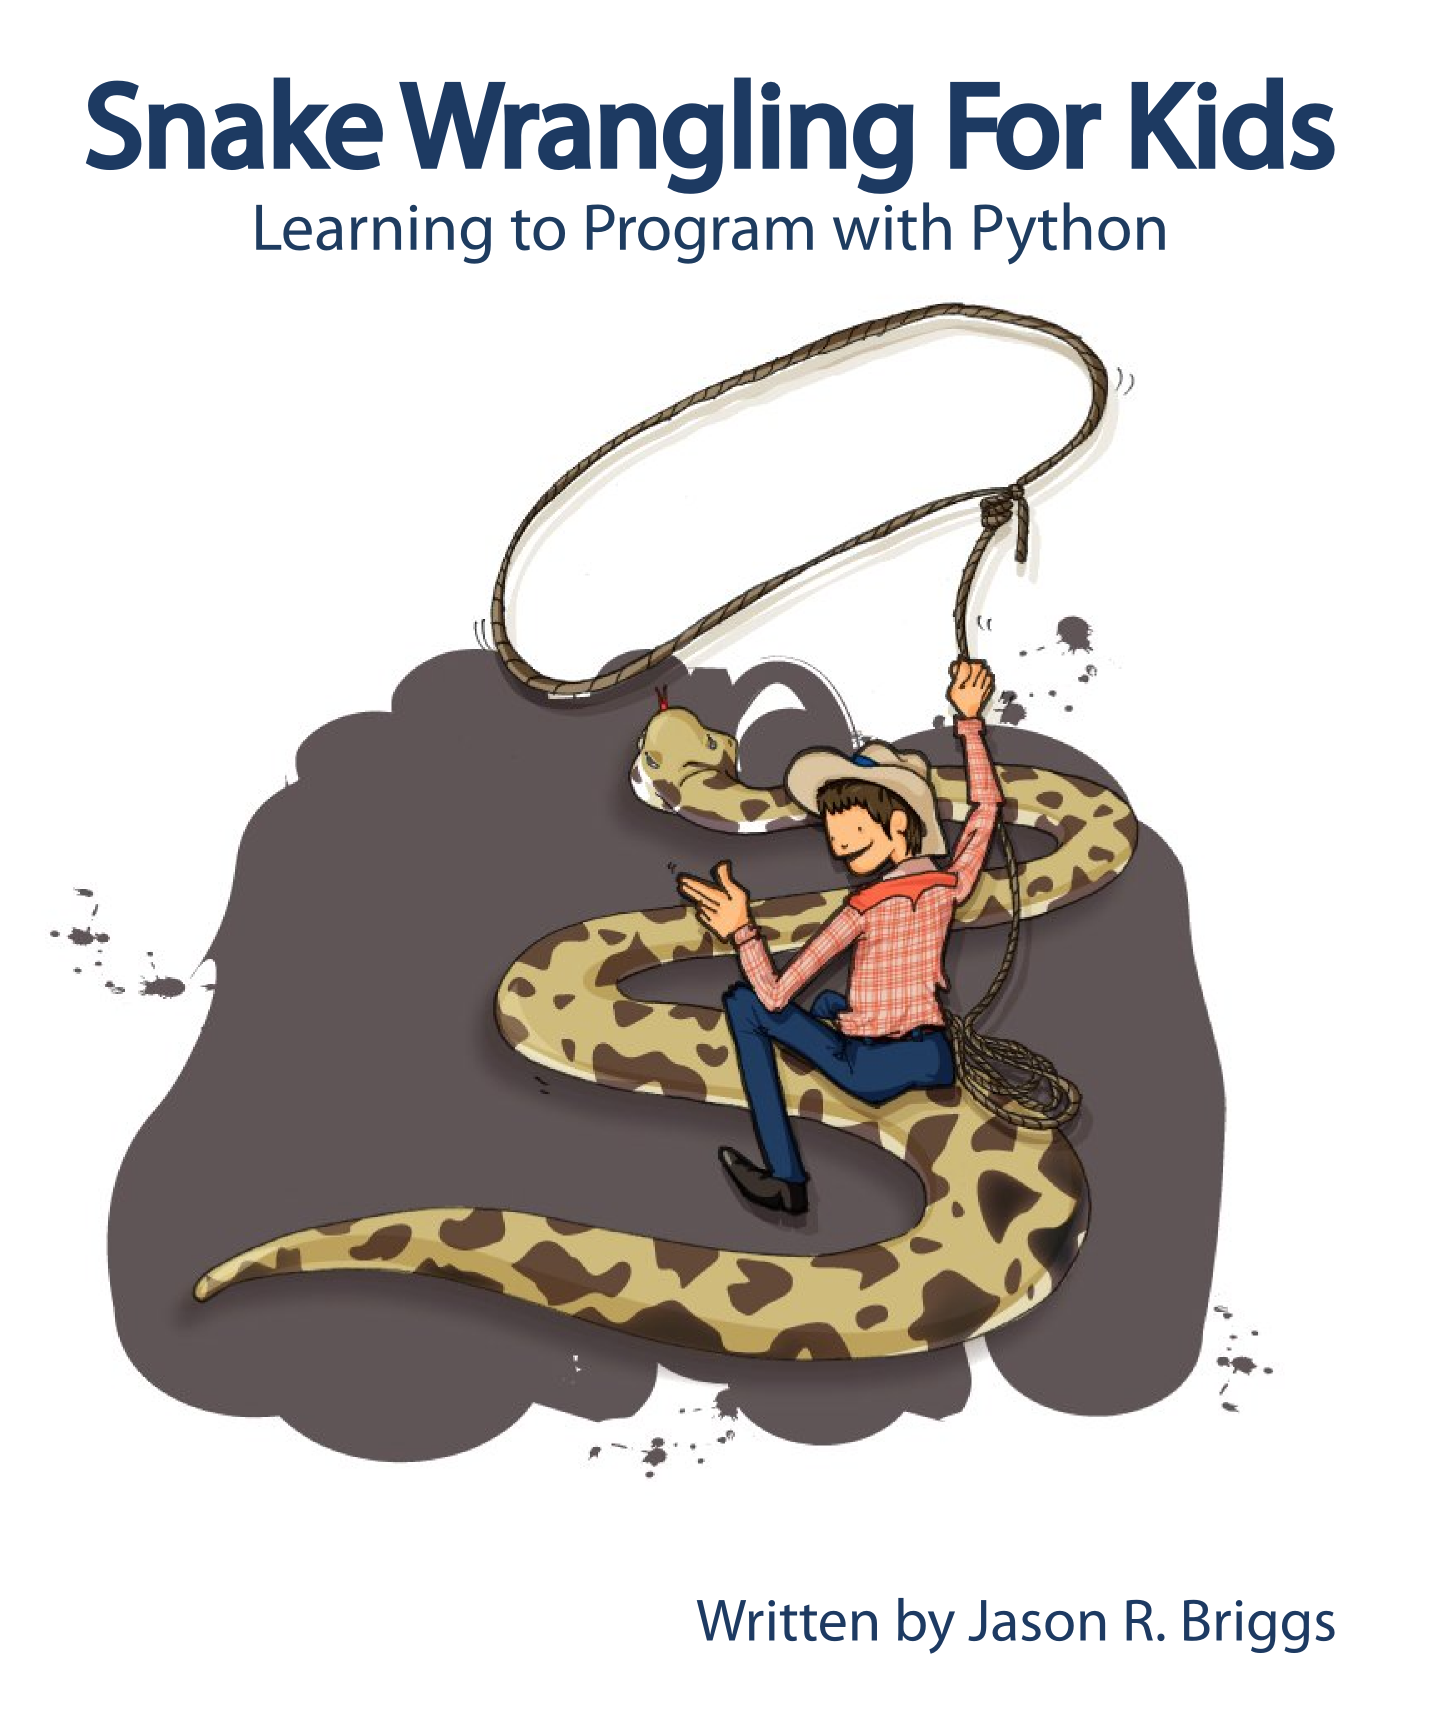
\includegraphics[width=0.9\paperwidth]{../en/cover.eps}
\end{textblock*}
\begin{flushright}
\vspace{30mm}

\includegraphics[width=40mm]{../en/linux-edition.eps} 
\end{flushright}
\end{titlepage}
%todo Finish translation
\noindent
\textsf{\emph{Snake Wrangling for Kids, Learning to Program with Python}}\\
by Jason R. Briggs\\
перевод на русский язык:\\
Кочетов Е.\,М. <Egor.Kochetoff@gmail.com>\\
\\
Version 0.7.7
\\\\
Copyright \copyright 2007, 2015\\
\\
Cover art and illustrations by Nuthapitol C.\\
\\
\noindent
\textsf{\emph{This book has been completely rewritten and updated, with new chapters (including developing graphical games), and new code examples. It also includes lots of fun programming puzzles to help cement the learning. Published by No Starch Press - available here: \href{http://nostarch.com/pythonforkids}{Python for Kids}. Also find more info \href{http://jasonrbriggs.com/python-for-kids/}{here}.}}
\\
\\
\linebreak
\noindent
Website:\\ \href{http://www.briggs.net.nz/log/writing/snake-wrangling-for-kids}{http://www.briggs.net.nz/log/writing/snake-wrangling-for-kids}\\
Github с переводом книги: \url{https://github.com/gluk47/swfk/tree/master/ru}\\
\\
\noindent
Thanks To:\\
Guido van Rossum (for benevolent dictatorship of the Python language), the members of the \href{http://www.python.org/community/sigs/current/edu-sig/}{Edu-Sig} mailing list (for helpful advice and commentary), author \href{http://www.davidbrin.com/}{David Brin} (the original \href{http://www.salon.com/tech/feature/2006/09/14/basic/}{instigator} of this book), Michel Weinachter (for providing better quality versions of the illustrations), and various people for providing feedback and errata, including: Paulo J. S. Silva, Tom Pohl, Janet Lathan, Martin Schimmels, and Mike Cariaso (among others).  Anyone left off this list, who shouldn't have been, is entirely due to premature senility on the part of the author.\\

\noindent
License:\\
\\

\includegraphics[width=40mm]{../en/by-nc-sa.eps}\\
This work is licensed under the Creative Commons Attribution-Noncommercial-Share Alike 3.0 New Zealand License. To view a copy of this license, visit\\ \href{http://creativecommons.org/licenses/by-nc-sa/3.0/nz/}{http://creativecommons.org/licenses/by-nc-sa/3.0/nz/} or send a letter to Creative Commons, 171 Second Street, Suite 300, San Francisco, California, 94105, USA.\\

\noindent
Ниже приведены основные положения лицензии.\\

\noindent
Лицензия позволяет:
\begin{itemize}
 \item \textbf{Делиться} — копировать, распространять и передавать эту работу,
 \item \textbf{Изменять} — адаптировать эту работу.
\end{itemize}
\noindent
На следующих условиях:
\begin{description}
 \item[Attribution.] Обязательно явно указать авторство этой работы таким способом, как этого просит автор (и так, чтобы не казалось, что автор прямо поддерживает вас или вашу работу, основанную на его).
 \item[Noncommercial.] Нельзя использовать эту работу и основанные на ней в коммерческих целях.
 \item[Share Alike.] Если вы изменяете, перерабатываете, адаптируете и распространяете эту работу, обязательно распространять её на условиях этой же лицензии.
\end{description}

\noindent
При любом использовании и распространении необходимо донести до получателей условия лицензии на эту работу.\\

\noindent
Any of the above conditions can be waived if you get permission from the copyright holder.\\

\noindent
Nothing in this license impairs or restricts the author's moral rights.\\

\vspace*{4cm}
\begin{center}

\includegraphics[width=5cm]{../en/python-powered.eps}
\end{center}

\mainmatter

\pagestyle{plain}

\pagenumbering{roman}
\tableofcontents
